
Lo scopo di questo capitolo è quello di riassumere gli esperimenti condotti.\newline
\indent Una volta individuati i tool capaci di determinare bound espliciti ai consumi di gas si è testato il loro comportamento su input diversi. Per dedurre la completezza del software, i programmi in input sono stati scelti in modo da testare diversi costrutti base messi a disposizione dal linguaggio Solidity.\newline
\indent I test sono stati condotti con il tool GASTAP e con il compilatore solc, ad oggi gli unici capaci di produrre dei bound ai consumi di gas per gli smart contract di Ethereum. Per quanto riguarda il primo gli sviluppatori hanno fornito i dettagli della sua implementazione, documentando in che modo venga condotta la loro analisi. Conoscere le tecniche utilizzate ha permesso di dedurre alcune proprietà del tool e dell'analisi di smart contract in generale. Dall'altro lato la documentazione ~\cite{solidity-docs} del compilatore solc tratta l'analisi del gas in modo superficiale. Tuttavia il suo impiego nei test condotti ci ha permesso di confrontare i risultati di GASTAP, in modo da considerare l'analisi degli smart contract in chiave critica.\newline

\newpage

\section{Caratteristiche del Tool GASTAP}

GASTAP (acronimo per Gas-Aware Smart contracT Analysis Platform ~\cite{DBLP:journals/corr/abs-1811-10403}), è un tool automatico di analisi statica per i programmi di Ethereum. La principale tecnica di analisi adottata da questo software è la Control Flow Analysis (vedi sez. 2.2.5).\newline
\indent Dato in input uno smart contract scritto in Solidity, EVM bytecode oppure EVM disassemblato, GASTAP produce un upper bound in termini di gas per ciscuna delle funzioni pubbliche che lo compongono. Per produrre questo calcolo il tool effettua una serie di operazioni in sequenza: (1) costruzione dei grafi \textit{control-flow} (CFG), (2) decompilazione del codice di basso livello in una rappresentazione di alto livello, (3) deduzione delle relazioni di grandezza, (4) generazione delle equazioni di gas, e (5) risoluzione delle equzioni fino a formare un bound.\newline
\indent GASTAP ha un ampio spettro di applicazioni, sia per chi sviluppa o possiede i contratti, sia per gli attaccanti, permettendo di individuare vulnerabilità nel codice e di verificare gli utilizzi di gas, eventualmente anche a scopo di debugging.
Dal punto di vista degli sviluppatori e dei proprietari un buon tool di analisi serve a conoscere la quantità di gas necessaria per eseguire in modo \textit{sicuro} il programma, garantendone la proprietà di liveness. Un altro beneficio è quello di poter determinare quante unità di gas investire per eseguire con successo una callback nei casi in cui uno smart contract si appoggi ad un servizio esterno.
Dal punto di vista degli attaccanti invece è possibile stimare quanto Ether è necessario investire per eseguire un attacco DoS, sebbene tali quantità siano svantaggiose dal punto di vista economico, rendendo poco invitante l'alternativa di compromettere uno smart contract.\newline

    \subsection{Struttura del TOOL}
    
    Per implementare ciascuna dele operazioni elencate sopra GASTAP si appoggia ad altri tool open-source. Questi, grazie a degli adattamenti, vengono utilizzati in sequenza al fine di realizzare l'architettura rappresentata in figura \ref{fig:gstp-struct}.\newline 
    
    \begin{figure}[h]
        \centering
        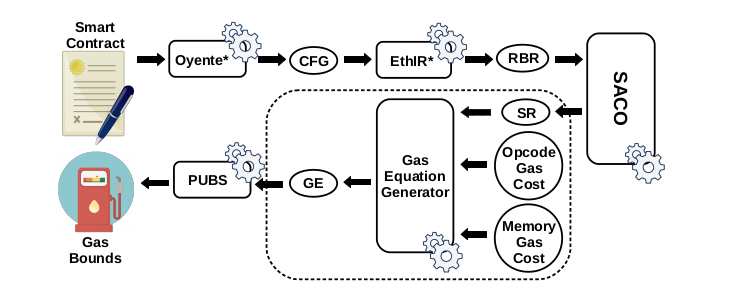
\includegraphics[scale=0.5]{GASTAP-structure.png}
        \caption{Architettura di GASTAP}
        \label{fig:gstp-struct}
    \end{figure}
    
    \begin{enumerate}
        \item \textbf{costruzione dei grafi control-flow (CFG)}: tale passaggio è realizzato con \textsc{oyente*}, un'estensione di ~\cite{melonproject/oyente}.
        \item \textbf{decompilazione del codice di basso livello}: in questa fase il bytecode viene tradotto in una RBR (\textit{Rule-Based Representation}) grazie ad \textsc{ethir*}, estensione del già citato ~\cite{albert2018ethir}.
        \item \textbf{deduzione delle relazioni di grandezza}: questo passaggio consiste nell'associare a ciascuna delle istruzioni in forma RBR le dimensioni dei dati con i quali interagisce. Quest'operazione è indispensabile per poter costruire le equazioni necessarie a calcolare i bound, e viene realizzata dal tool SACO ~\cite{10.1007/978-3-642-54862-8_46}, che produce le così dette SR (\textit{Size Relations}).
        \item \textbf{generazione delle equazioni di gas}: costituisce il core di GASTAP. Al fine di produrre le equazioni, il tool utilizza le SR insieme alla codifica dei costi delle istruzioni EVM, secondo le specifiche di \cite{wood2014ethereum}. Questi vengono suddivisi tra i costi richiesti dall'esecuzione del bytcode (\textit{Opcode Gas Cost}) e quelli richiesti per l'uso della memoria (\textit{Memory Gas Cost}). 
        \item \textbf{risoluzione delle equazioni fino a formare un bound}: per produrre il risultato finale GASTAP utilizza il solver PUBS ~\cite{albert2008automatic}, che risolve le GE (\textit{Gas Equations}) producendo una formula chiusa dei costi in termini di gas. 
    \end{enumerate}

    \subsection{Interfaccia Web}
    
    GASTAP è utilizzabile tramite un'interfaccia web, disponibile all'indirizzo \\
    https://costa.fdi.ucm.es/gastap.
    
    \begin{figure}[h]
        \centering
        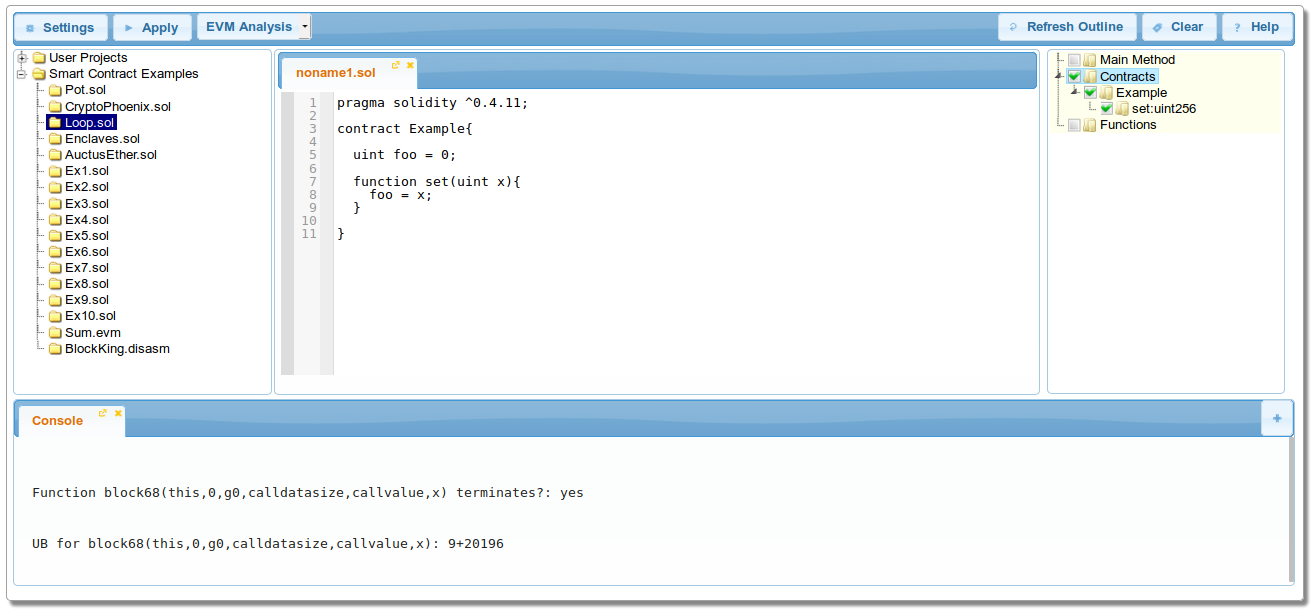
\includegraphics[scale=0.3]{GASTAP-example.png}
        \caption{Interfaccia di GASTAP}
        \label{fig:gstp-example}
    \end{figure}
    
    \`E possibile scrivere un proprio programma in Solidity oppure scegliere uno degli esempi proposti dal menù ``Smart Contract Examples''.\newline
    \indent Una volta selezionato il programma di input, cliccando su ``Refresh Outline'' GASTAP mappa le funzioni pubbliche del nostro programma, che vengono mostrate nella sezione di destra. Dopo aver selezionato i metodi che si vogliono analizzare, il pulsante ``Apply'' esegue l'analisi e produce un output nella Console.\newline
    \indent Nell'esempio viene proposto un semplice programma che setta una variabile globale. Stando all'output prodotto, tale programma è garantito teminare, e l'\textit{Upper Bound} (UB) ai consumi di gas è \verb|9+20196| .

    

    
\section{Compilatore solc}

Si tratta del compilatore ufficiale del linguaggio Solidity, utilizzabile da linea di comando.\newline
\indent Il comando \verb|solc --help| fornisce la spiegazione di ciascuna delle opzioni con cui può essere lanciato.

\lstset{
    style=cmd-line,
    literate={~} {$\sim$}{1}
}

\begin{lstlisting}
$~solc --help

solc, the Solidity commandline compiler.

This program comes with ABSOLUTELY NO WARRANTY. This is free software, and you
are welcome to redistribute it under certain conditions. See 'solc --license'
for details.

Usage: solc [options] [input_file...]

...

Allowed options:
  --help               Show help message and exit.
  --version            Show version and exit.
  --license            Show licensing information and exit.
    
\end{lstlisting}    
    
\ldots

\begin{lstlisting}[frame=single, 
                    framerule=0pt]

  --gas                Print an estimate of the  
                       maximal gas usage for each 
                       function. 
 
\end{lstlisting}


\ldots

\begin{lstlisting}

  --link               Switch to linker mode,            
                       ignoring all options apart from --libraries and modify  binaries in place.

\end{lstlisting}

Per condurre i nostri test abbiamo utilizzato il compilatore con l'opzione \verb|--gas|. Ecco un esempio del suo utilizzo sul programma raffigurato in figura \ref{fig:gstp-example}.

\begin{lstlisting}
$~solc --gas example.sol 

======= example.sol:Example =======
Gas estimation:
construction:
   5093 + 32800 = 37893
external:
   set(uint256):	20205

\end{lstlisting}

Confrontando i risultati ottenuti con quelli prodotti da GASTAP si evince che la stima del gas consumato dalla funzione \verb|set()| corrisponde a quela determinata da solc. Dunque l'uso dell'analisi statica non fa sì che si perda accuratezza nel calcolo.\newline
\indent Nella sezione 4.3.2 l'esempio verrà ripreso al fine di comprendere il bound.\newline


\section{Test Condotti}



    \subsection{Caso di Studio: CryptoPhoenix.sol}

    \subsection{Operazioni di Assegnamento}

    \subsection{Costrutto for}
    
    \subsection{Cicli for Annidati}

    \subsection{Costrutto while}
    
        \subsubsection{while.sol}

        \subsubsection{sqrt.sol}

    \subsection{Ricorsione}

        \subsubsection{Ricorsione Diretta}

        \subsubsection{Ricorsione Indiretta}
        
        \subsubsection{Ricorsione Multipla}
    
\section{Risultati}

